% 原书第4章PDF第1—11页（止于4.1.3.6标题之前），印刷247—257页。
\chapter{RNA 测序数据分析}
\label{ch:rna-seq}
\section{RNA 测序数据分析中的标准化方法}
\subsection{基因表达}

RNA 是一类动态且多样的生物分子。基因表达（gene expression）在多种生物学过程中发挥重要作用。基因中的信息编码在核苷酸序列中；基因表达通过信使 RNA（messenger RNA，mRNA），将基因所含的 DNA 信息转化为蛋白质的产生（\url{https://www2.stat.duke.edu/courses/Spring04/sta278/refinfo/Gene_Expression.pdf}）。mRNA 与 DNA 有义链的序列相同，只是以 U 替代 T，同时与模板链互补（图4.1a）。

转录过程包括三个基本步骤。第一步，转录因子（transcription factor）与启动子中的结合位点相互作用，引导 RNA 聚合酶（图4.1b）。其他转录因子还可结合到位于基因更上游或下游的增强子上（图4.1b）。第二步，聚合酶 II（基础转录装置）必须从基因中的特定位点启动转录；该起始位点由 RNA 聚合酶与转录因子共同决定。第三步，聚合酶完成并终止该基因的转录。转录终止可在基因的一个较宽区域内发生，终止位置具有异质性。

转录起始的调控是基因控制的关键步骤。它主要通过调控转录因子与启动子、增强子中顺式作用序列之间的相互作用，决定 RNA 聚合酶与基因结合并进行转录的频率。

转录开始后，RNA 加工随之进行，包括对蛋白质编码转录本作剪接、连接外显子序列，以及去除内含子序列（图4.2）。剪接反应首先识别 RNA 剪接位点连接处的特定序列，然后在外显子 $3'$ 端与内含子 $5'$ 端的交界处切开 RNA，再在内含子 $3'$ 端切开，使两个外显子得以连接。图4.3展示了剪接产生两种 mRNA 异构体（isoform）的过程：mRNA1 由外显子1与外显子3连接形成；mRNA2 则由外显子1、外显子2和外显子3全部连接形成。

\begin{figure}[htbp]
\centering
\begin{tikzpicture}[x=1cm,y=1cm,>=Stealth,font=\small]
\fill[red!90] (1.2,5.5) rectangle (6.2,5.95);
\node[text=white,font=\bfseries] at (3.7,5.72) {AA GTGTT};
\fill[green!65!black] (1.2,4.8) rectangle (6.2,5.2);
\node at (.9,5.72) {$5'$};\node at (.9,5) {$3'$};
\node[anchor=west] at (6.4,5.72) {有义链};
\node[anchor=west] at (6.4,5) {$5'$ 模板链};
\draw[->,very thick,inkblue] (3.7,4.75)--(3.7,4.1);
\fill[red!90] (1,3.55) rectangle (6,4);
\node[text=white,font=\bfseries] at (3.5,3.77) {AA GUGUU};
\node at (.7,3.77) {$5'$};
\node[anchor=west] at (6.2,3.77) {$3'$ 转录产物};
\node at (.7,3.05) {(a)};
\draw[red,->] (.6,.2)--(7.35,.2);
\filldraw[fill=inkblue!65,draw=inkblue] (1.5,.2) rectangle (2.2,.6);
\filldraw[fill=inkblue!65,draw=inkblue] (2.5,.2) rectangle (3.2,.6);
\filldraw[fill=inkblue!65,draw=inkblue] (4.6,.2) rectangle (5.3,.6);
\filldraw[fill=inkblue!65,draw=inkblue] (5.5,.2) rectangle (6.2,.6);
\filldraw[fill=inkblue!65,draw=inkblue] (6.4,.2) rectangle (7.1,.6);
\filldraw[fill=green!65!black] (7.4,0) rectangle (11.7,.55);
\node at (2.3,.95) {增强子};\node at (5.8,.95) {启动子};
\node at (8.9,.95) {外显子};
\node[ellipse,draw=inkblue,fill=inkblue!65,minimum width=.9cm,minimum height=1.05cm] (ch04atf) at (4.9,2.35) {};
\node[anchor=west] at (5.6,2.4) {转录因子};
\draw[red,->] (ch04atf.south)--(4.9,.65);
\draw[red,->] (7.4,.55)--(7.4,1.8)--(10.1,1.8);
\node[anchor=west,align=left] at (8.2,2.35) {基础转录\\装置};
\node at (.7,-.25) {(b)};
\end{tikzpicture}
\origfig{1}{转录过程。}
\label{fig:ch04a-01}
\end{figure}

\begin{figure}[htbp]
\centering
\begin{tikzpicture}[x=1cm,y=1cm,>=Stealth,font=\small]
\node[font=\bfseries] at (6,5.5) {基因结构};
\draw[red,thick] (.9,2.5)--(12.5,2.5);
\foreach \x/\w in {2.9/2,5.7/1.6,9/2}{
 \draw[magenta] (\x,2.95) rectangle ++(\w,.45);
}
\fill[green!60!black] (3.45,2.95) rectangle (4.9,3.4);
\fill[green!60!black] (5.7,2.95) rectangle (7.3,3.4);
\fill[green!60!black] (9,2.95) rectangle (10.45,3.4);
\node[draw,align=center,font=\bfseries,inner sep=4pt] (ch04aprom) at (1.5,4.45) {启动子\\区域};
\draw[magenta,->] (ch04aprom.south)--(1.5,2.6);
\node[draw,font=\bfseries,inner sep=4pt] at (7.1,4.7) {外显子（填充与未填充的框区域）};
\draw[magenta] (2.9,4.25)--(11,4.25);
\foreach \x in {3.9,6.5,10}{\draw[magenta,->] (\x,4.25)--(\x,3.5);}
\node[draw,inner sep=2pt] at (2.9,2.5) {$+1$};
\node[text=orange!85!black] at (7.1,1.95) {内含子（位于外显子之间）};
\draw[magenta,->] (5.25,1.95)--(5.25,3.05);
\draw[magenta,->] (8.15,1.95)--(8.15,3.05);
\draw[inkblue,<->,thick] (2.75,1.55)--(11,1.55);
\node[draw,text=inkblue,fill=white,font=\bfseries] at (7,1.2) {转录区域};
\node[font=\bfseries,anchor=west] at (.9,.3) {mRNA 结构};
\draw (4.1,-.4) rectangle (10.2,0);
\filldraw[fill=green!60!black] (4.7,-.4) rectangle (6.4,0);
\filldraw[fill=green!60!black] (6.4,-.4) rectangle (7.95,0);
\filldraw[fill=green!60!black] (7.95,-.4) rectangle (9,0);
\node at (3.7,-.2) {$5'$};\node at (10.6,-.2) {$3'$};
\draw[<->,thick] (4.7,-.75)--(9,-.75);
\node[font=\bfseries] at (6.85,-1.1) {翻译区域};
\end{tikzpicture}
\origfig{2}{RNA 加工。}
\label{fig:ch04a-02}
\end{figure}

\begin{figure}[htbp]
\centering
\begin{tikzpicture}[x=1cm,y=1cm,>=Stealth,font=\small]
\fill[red!90] (1.6,2.3) rectangle (3.3,3.9);
\filldraw[fill=inkblue!70,draw=blue] (4.65,2.3) rectangle (5.7,3.9);
\fill[green!65!black] (7.15,2.3) rectangle (9.25,3.9);
\node[text=white] at (2.45,3.1) {CTAG};
\node[text=white] at (5.18,3.1) {GA};
\node[text=white] at (8.2,3.1) {GAT};
\node[text=red] at (2.35,1.95) {外显子1};
\node[text=inkblue] at (5.18,4.3) {外显子2};
\node[text=green!65!black] at (8.35,1.95) {外显子3};
\draw[magenta,<->] (2.45,3.95)--(2.45,4.9)--(7.95,4.9)--(7.95,3.95);
\draw[inkblue,<->] (2.95,2.3)--(2.95,1.7)--(4.65,1.7)--(4.65,2.3);
\draw[inkblue,<->] (5.55,2.3)--(5.55,1.7)--(7.45,1.7)--(7.45,2.3);
\node[anchor=east] at (1.85,.75) {转录本};
\node[text=red,font=\bfseries] at (2.6,.75) {CTAG};
\draw[orange] (3.35,.75)--(7.45,.75);
\node[text=green!65!black,font=\bfseries] at (8.15,.75) {GAT};
\node[anchor=west] at (9.1,.75) {mRNA1};
\node[text=red,font=\bfseries] at (2.6,-.15) {CTAG};
\draw[orange] (3.35,-.15)--(4.7,-.15);
\node[text=inkblue,font=\bfseries] at (5.18,-.15) {GA};
\draw[orange] (5.7,-.15)--(7.45,-.15);
\node[text=green!65!black,font=\bfseries] at (8.15,-.15) {GAT};
\node[anchor=west] at (9.1,-.15) {mRNA2};
\end{tikzpicture}
\origfig{3}{剪接。}
\label{fig:ch04a-03}
\end{figure}


转录的最后一步是通过多聚腺苷酸化，在 RNA 的 $3'$ 末端加上200个腺苷残基。该 poly A 为参与蛋白质合成的蛋白质提供结合位点，并保护 RNA 免于降解。转录本在细胞核内产生；最终加工产物 mRNA 从细胞核运输至细胞质，在核糖体的帮助下被翻译为蛋白质。
\FloatBarrier

\subsection{RNA 测序表达谱分析}

尽管复杂疾病遗传研究已取得很大进展，关联研究所识别遗传变异的功能信息仍然有限。基因表达变异会引起表型变异，因此，基因表达分析是研究遗传变异功能的重要信息来源，在揭示复杂性状机制方面发挥着日益重要的作用。下一代测序（next-generation sequencing，NGS）技术推动了转录组研究的革新。新近发展的深度测序技术，正成为基因表达谱分析的首选平台。RNA 测序（RNA sequencing，RNA-seq）通过测量样本中全部基因的 mRNA 水平，提供转录组的全面图景，因而是刻画转录全局变化的一种有吸引力的选择（Hong et al. 2013）。

与微阵列相比，RNA-seq 技术在基因表达的定性与定量分析方面均有显著改进（Zyprych-Walczak et al. 2015）。第一，RNA-seq 提供多层次的分辨率和转录组复杂性信息，包括外显子、SNP 与基因组位置层面的表达，剪接，整个基因范围内的转录后 RNA 编辑，以及异构体表达和等位基因特异性表达。第二，RNA-seq 数据的背景噪声更低，检测动态范围更大（Hrdlickova et al. 2017）。第三，RNA-seq 能够检测可变剪接异构体。

生成 RNA-seq 数据时，首先从 RNA 样本中提取全部 mRNA，将其打断并反转录，构建带有接头的 cDNA 片段文库（图4.4）。这些短 cDNA 片段经聚合酶链式反应扩增后，由测序仪测序，产生数百万条短读段。随后，将读段比对到参考基因组或参考转录本，以目标区域内的读段数度量丰度。即使没有基因组序列，也可对读段作从头组装，构建转录图谱（Li and Xiong 2015）。

\begin{figure}[p]
\centering
\begin{tikzpicture}[x=1cm,y=1cm,>=Stealth,font=\small]
\filldraw[draw=inkblue,fill=inkblue!65] (1,11.8) rectangle (9.6,12);
\filldraw[draw=inkblue,fill=red!90] (9.6,11.65) rectangle (12.2,12.1);
\node[text=white] at (10.9,11.87) {AAAAAAA};
\draw[green!70!black,very thick,->] (5.8,11.6)--(5.8,10.8);
\node at (2.9,11.2) {打断};
\node[anchor=west] at (10.3,10.8) {200--300 bp};
\foreach \x/\y in {1.4/10.7,2.2/10.95,3.7/10.7,4.2/10.95,6.5/10.8,7/11.05,8.4/10.8,8.9/11.05}
 \filldraw[draw=inkblue,fill=inkblue!65] (\x,\y) rectangle ++(1,.12);
\node at (3.2,10.2) {RNA 片段};
\foreach \x in {1,4.2,7.4}{
 \fill[red!90] (\x,9.5) rectangle ++(.8,.15);
 \filldraw[draw=inkblue,fill=inkblue!65] (\x+.8,9.5) rectangle ++(1,.15);
 \fill[red!90] (\x+1.8,9.5) rectangle ++(.8,.15);
 \fill[red!90] (\x,9.25) rectangle ++(.8,.15);
 \filldraw[draw=inkblue,fill=inkblue!65] (\x+.8,9.25) rectangle ++(1,.15);
 \fill[red!90] (\x+1.8,9.25) rectangle ++(.8,.15);
}
\node[text=red,anchor=east] at (.9,9.3) {接头};
\draw[green!65!black,->] (.45,9.5)--(1,9.6);
\node[anchor=west] at (10.25,9.45) {构建测序文库};
\node[anchor=east] at (.7,8) {基因};
\foreach \x in {1,4.5,8.3} \fill[green!65!black] (\x,7.95) rectangle ++(2.5,.2);
\foreach \x/\y in {1.2/7.3,1.4/7.05,2.1/7.55,2.5/6.8,3/7.1,4.45/7.55,4.6/7.15,5.35/6.9,5.8/7.5,6/7.1,8.4/7.15,8.9/7.5,9/6.9,10/7.1}
 \filldraw[draw=inkblue,fill=inkblue!65] (\x,\y) rectangle ++(1,.12);
\draw[green!65!black,dashed] (3.1,7.6)--(4.45,7.6);
\draw[green!65!black,dashed] (4,7.15)--(4.6,7.2);
\draw[green!65!black,dashed] (7,7.15)--(8.4,7.2);
\node[anchor=west] at (11.1,7.35) {剪接感知比对};
\node[anchor=east] at (.7,6.1) {基因组};
\fill[magenta!65] (1,6) rectangle (10.8,6.2);
\node[anchor=south west,inner sep=0] at (1,.0) {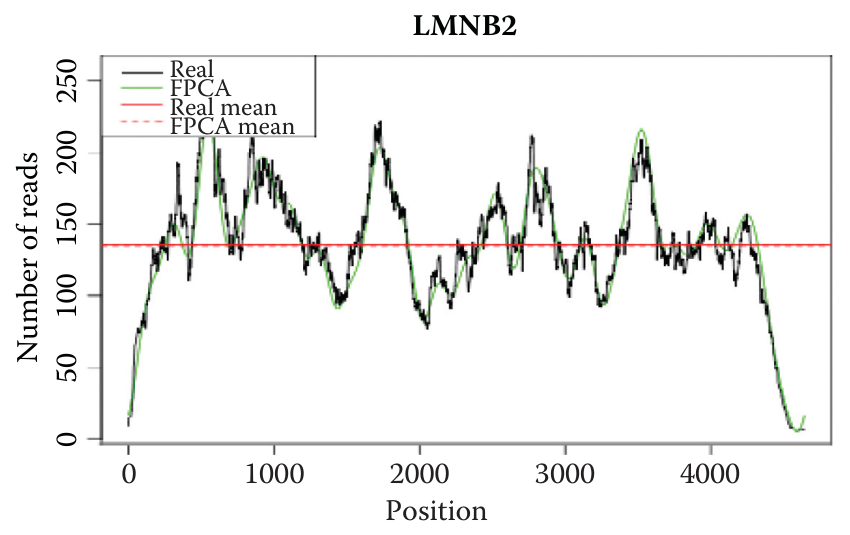
\includegraphics[width=9.4cm]{figures/ch04a_fig04_data.png}};
\node[anchor=west] at (10.7,3.2) {RNA 表达水平};
\fill[white] (5.224254595588236,0.06083399155560662) rectangle (6.4288921616498165,0.44789281508501844);
\node[font=\scriptsize,rotate=0,inner sep=0] at (5.826573378619026,0.25436340332031254) {位置};
\fill[white] (1.1239476336310892,1.876407434800092) rectangle (1.5220652806899126,4.262682387408089);
\node[font=\scriptsize,rotate=90,inner sep=0] at (1.323006457160501,3.0695449111040904) {读段数};
\filldraw[fill=white,draw=gray] (2.072705882352942,4.25764705882353) rectangle (4.621764705882353,5.3635294117647065);
\draw[black,solid,thin] (2.192705882352942,5.233529411764707)--(2.572705882352942,5.233529411764707);
\node[font=\tiny,anchor=west,inner sep=0] at (2.6427058823529417,5.233529411764707) {观测};
\draw[green!65!black,solid,thin] (2.192705882352942,4.993529411764706)--(2.572705882352942,4.993529411764706);
\node[font=\tiny,anchor=west,inner sep=0] at (2.6427058823529417,4.993529411764706) {FPCA};
\draw[red,solid,thin] (2.192705882352942,4.753529411764706)--(2.572705882352942,4.753529411764706);
\node[font=\tiny,anchor=west,inner sep=0] at (2.6427058823529417,4.753529411764706) {观测均值};
\draw[red,dashed,thin] (2.192705882352942,4.513529411764707)--(2.572705882352942,4.513529411764707);
\node[font=\tiny,anchor=west,inner sep=0] at (2.6427058823529417,4.513529411764707) {FPCA均值};
\end{tikzpicture}
\origfig{4}{RNA-seq 表达谱分析。}
\label{fig:ch04a-04}
\end{figure}

\FloatBarrier

\subsection{标准化方法}

RNA-seq 数据结构复杂，因而估计 mRNA 丰度并不简单。分析方法是准确解释数据的关键（Li et al. 2015）。数据中常可观察到多种伪影和偏倚，影响由 RNA-seq 数据得到的表达定量。因此，标准化（normalization）是后续 RNA-seq 分析中的关键步骤，例如基因差异表达、eQTL 分析和基因调控网络分析等。标准化旨在识别并去除数据中样本间系统性的技术差异，尽可能消除技术偏倚。目前已发展出多种 RNA-seq 标准化方法，包括原始计数（raw count，RC）、上四分位数（upper quartile，UQ）、中位数（median，Med）、M 值截尾均值（trimmed mean of M-value，TMM）标准化（Robinson and Oshlack 2010）、DESeq（Anders and Huber 2010）、分位数（quantile，Q）标准化（Bolstad et al. 2003）、每百万比对读段中的每千碱基读段数（RPKM）（Mortazavi et al. 2008）、基于期望最大化的 RNA-seq 定量方法 RSEM（Li et al. 2011），以及 Sailfish（Patro et al. 2014）。

标准化的主要原因，是不同样本的比对读段总数不同。先考虑全局标准化方法：对每个样本 $j$，用一个因子 $C_j$ 缩放全部基因的计数。其目的是使测序深度不同的样本，其读段计数具有可比性。定义
\[
\begin{aligned}
n_{gj}:&\quad\text{样本 }j\text{ 中基因 }g\text{ 的观测计数},\\
D_j=\sum_{g=1}^{G}n_{gj}:&\quad\text{样本 }j\text{ 的读段总数，}G\text{ 为基因数},\\
C_j:&\quad\text{样本 }j\text{ 对应的标准化因子}.
\end{aligned}
\]

\subsubsection{总读段计数标准化}

假设读段计数与表达水平及测序深度成正比。数据标准化要求缩放后每个样本的读段总数相等，因此应选择标准化因子，使
\begin{equation}
C_1D_1=\cdots=C_ND_N=10^6,
\tag{4.1}
\end{equation}
其中 $N$ 是样本总数。样本 $j$ 的标准化因子计算为
\begin{equation}
C_j=\frac{10^6}{D_j}.
\tag{4.2}
\end{equation}
基因 $g$ 的标准化读段计数为
\begin{equation}
n_{gj}^*=C_jn_{gj}=\frac{n_{gj}}{D_j}10^6.
\tag{4.3}
\end{equation}
也就是说，先用转录本的读段计数除以读段总数，再缩放至每百万读段的计数。

\begin{bookexample}{4.1}
考虑表4.1中的简单例子：有3个样本及10个基因的观测计数。由于基因数较少，以100替代100万。每个基因的标准化读段计数用式 (4.3) 计算，标准化因子与标准化数据汇总于表4.1。
\end{bookexample}
\begin{table}[htbp]
\centering
\origtable{1}{原始与标准化后的读段计数。}
\label{tab:ch04a-01}
\small
\setlength{\tabcolsep}{5pt}
\begin{tabular}{lrrrrrr}
\toprule
&\multicolumn{3}{c}{原始数据}&\multicolumn{3}{c}{标准化数据}\\
\cmidrule(lr){2-4}\cmidrule(lr){5-7}
&NA19099&NA18510&NA18520&NA19099&NA18510&NA18520\\
\midrule
 & 26 & 13 & 27 & 11.76 & 12.87 & 15.25\\
 & 15 & 7 & 15 & 6.79 & 6.93 & 8.47\\
 & 22 & 15 & 16 & 9.95 & 14.85 & 9.04\\
 & 3 & 0 & 8 & 1.36 & 0 & 4.52\\
 & 2 & 0 & 1 & 0.91 & 0 & 0.57\\
 & 11 & 11 & 17 & 4.98 & 10.89 & 9.6\\
 & 27 & 6 & 29 & 12.22 & 5.94 & 16.38\\
 & 85 & 28 & 38 & 38.46 & 27.72 & 21.47\\
 & 7 & 7 & 3 & 3.17 & 6.93 & 1.69\\
 & 23 & 14 & 23 & 10.41 & 13.86 & 12.99\\
合计 & 221 & 101 & 177 & 100 & 100 & 100\\
标准化因子 & 0.4525 & 0.9901 & 0.565 & & &\\
\bottomrule
\end{tabular}
\end{table}


\subsubsection{上分位数标准化}

总读段计数标准化利用每个样本的读段总数，计算数据标准化所用的缩放因子，而不考虑样本读段计数的分布。为使基因读段计数在样本间的分布相匹配，发展了上分位数标准化方法（Bullard et al. 2010）。设 $Q_j^{(p)}$ 为样本 $j$ 的上分位数，即第 $p$ 百分位数。将式 (4.1) 中的 $D_j$ 替换为 $D_jQ_j^{(p)}$，得到
\begin{equation}
C_1D_1Q_1^{(p)}=\cdots=C_ND_NQ_N^{(p)}=C.
\tag{4.4}
\end{equation}
若假设常数 $C$ 等于几何均值 $\bigl(\prod_{l=1}^{N}D_lQ_l^{(p)}\bigr)^{1/N}$，则式 (4.4) 化为
\begin{equation}
\begin{aligned}
C_1D_1Q_1^{(p)}=\cdots=C_ND_NQ_N^{(p)}
&=\left(\prod_{l=1}^{N}D_lQ_l^{(p)}\right)^{1/N}\\
&=\exp\left\{\frac1N\sum_{l=1}^{N}\log\bigl(D_lQ_l^{(p)}\bigr)\right\}.
\end{aligned}
\tag{4.5}
\end{equation}
因此，样本 $j$ 的标准化因子计算为
\begin{equation}
C_j=\frac{\exp\left\{\frac1N\sum_{l=1}^{N}\log\bigl(D_lQ_l^{(p)}\bigr)\right\}}
{D_jQ_j^{(p)}}.
\tag{4.6}
\end{equation}
上分位数标准化通常取 $p=0.75$。

\subsubsection{相对对数表达量（RLE）}

标准化因子之比 $C_{j_1}/C_{j_2}$ 也可视为大小之比。如果基因 $g$ 不存在差异表达，或者样本 $j_1$ 与 $j_2$ 是重复样本，那么，同一基因 $g$ 在两个样本中的期望计数之比 $n_{gj_1}/n_{gj_2}$，应等于大小之比 $C_{j_1}/C_{j_2}$。上一小节用读段总数 $D_j$ 估计大小 $C_j$。但实际中常可发现，少数具有高度差异表达的基因，会对读段总数产生很大影响，使读段总数或期望计数比的估计出现偏倚。

将跨样本的几何均值 $\bigl(\prod_{l=1}^{N}n_{gl}\bigr)^{1/N}$ 作为伪参考样本的基因表达水平，并假设该伪参考样本中各基因的表达水平，等于该基因跨样本的几何均值，则有
\begin{equation}
\frac{n_{gj_1}}{n_{gj_2}}
=\frac{n_{gj_1}}{\left(\prod_{l=1}^{N}n_{gl}\right)^{1/N}}
=\frac{C_{j_1}}{C_{j_2}}.
\tag{4.7}
\end{equation}
若假设伪参考样本的标准化因子 $C_{j_2}=1$，则式 (4.7) 化为
\begin{equation}
C_{j_1}=\frac{n_{gj_1}}{\left(\prod_{l=1}^{N}n_{gl}\right)^{1/N}}.
\tag{4.8}
\end{equation}
对式 (4.8) 两边取中位数，得到
\begin{equation}
C_j=\underset{g}{\operatorname{median}}\frac{n_{gj}}{\left(\prod_{l=1}^{N}n_{gl}\right)^{1/N}}.
\tag{4.9}
\end{equation}
标准化因子之积应为1，因此，最终将标准化因子定义为
\begin{equation}
C_j=\frac{\exp\left(\frac1N\sum_{l=1}^{N}\log(C_l)\right)}{C_j}.
\tag{4.10}
\end{equation}
容易验证
\[
\prod_{j=1}^{N}C_j
=\frac{\exp\left(\sum_{l=1}^{N}\log(C_l)\right)}{\prod_{j=1}^{N}C_j}
=\frac{\prod_{j=1}^{N}C_j}{\prod_{j=1}^{N}C_j}=1.
\]

\begin{bookexample}{4.2}
在例4.1的三个 RNA-seq 样本中，标准化因子为 $C=[0.9039,1.1854,0.9333]$。表4.2给出标准化数据；与表4.1相比，标准化有所改善。
\end{bookexample}
\begin{table}[htbp]
\centering
\origtable{2}{使用 RLE 得到的原始与标准化读段计数。}
\label{tab:ch04a-02}
\small
\setlength{\tabcolsep}{5pt}
\begin{tabular}{lrrrrrr}
\toprule
&\multicolumn{3}{c}{原始数据}&\multicolumn{3}{c}{标准化数据}\\
\cmidrule(lr){2-4}\cmidrule(lr){5-7}
&NA19099&NA18510&NA18520&NA19099&NA18510&NA18520\\
\midrule
 & 26 & 13 & 27 & 23.5 & 15.41 & 25.2\\
 & 15 & 7 & 15 & 13.56 & 8.3 & 14\\
 & 22 & 15 & 16 & 19.89 & 17.78 & 14.93\\
 & 3 & 0 & 8 & 2.71 & 0 & 7.47\\
 & 2 & 0 & 1 & 1.81 & 0 & 0.93\\
 & 11 & 11 & 17 & 9.94 & 13.04 & 15.87\\
 & 27 & 6 & 29 & 24.4 & 7.11 & 27.07\\
 & 85 & 28 & 38 & 76.83 & 33.19 & 35.47\\
 & 7 & 7 & 3 & 6.33 & 8.3 & 2.8\\
 & 23 & 14 & 23 & 20.79 & 16.6 & 21.47\\
标准化因子 & 0.4525 & 0.9901 & 0.565 & 0.9039 & 1.1854 & 0.9333\\
\bottomrule
\end{tabular}
\end{table}


\subsubsection{M 值截尾均值（TMM）}

显然，读段总数在很大程度上取决于少数高表达基因。上一小节假设大多数基因没有差异表达。进行数据标准化之前，需要剔除表达最高和最低的基因。M 值截尾均值（TMM）过程，首先定义两个量：对数倍数变化与绝对强度。以 $r$ 表示参考样本。基因 $g$ 在样本 $j$ 相对于参考样本 $r$ 的对数倍数变化 $M_g(j,r)$，定义为
\begin{equation}
M_g(j,r)=\log_2\left(\frac{n_{gj}}{D_j}\right)-\log_2\left(\frac{n_{gr}}{D_r}\right).
\tag{4.11}
\end{equation}
基因 $g$ 的绝对强度 $A_g(j,r)$ 定义为
\begin{equation}
A_g(j,r)=\frac12\left[\log_2\left(\frac{n_{gj}}{D_j}\right)+\log_2\left(\frac{n_{gr}}{D_r}\right)\right].
\tag{4.12}
\end{equation}
剔除最极端的30\% $M_g$ 值与5\% $A_g$ 值后，令 $G^*$ 表示剩下具有有效 $M_g$、$A_g$ 值的基因集合。定义标准化统计量
\begin{equation}
\operatorname{TMM}(j,r)=\frac{\sum_{g\in G^*}W_g(j,r)M_g(j,r)}{\sum_{g\in G^*}W_g(j,r)},
\tag{4.13}
\end{equation}
其中权重 $W_g(j,r)$ 定义为对数倍数变化 $M_g(j,r)$ 方差的倒数。可以证明，其方差近似为（习题4.2）
\[
\Var\bigl(M_g(j,r)\bigr)=\frac{D_j-n_{gj}}{D_jn_{gj}}+\frac{D_r-n_{gr}}{D_rn_{gr}}.
\]
所以，权重为
\begin{equation}
W_g(j,r)=\left(\frac{D_j-n_{gj}}{D_jn_{gj}}+\frac{D_r-n_{gr}}{D_rn_{gr}}\right)^{-1}.
\tag{4.14}
\end{equation}
样本 $j$ 的标准化因子定义为
\begin{equation}
C_j=2^{\operatorname{TMM}(j,r)}.
\tag{4.15}
\end{equation}
最后，为使各标准化因子之积等于1，将标准化因子 $C_j$ 定义为
\begin{equation}
C_j=\frac{\exp\left(\frac1N\sum_{l=1}^{N}\log(C_l)\right)}{C_j}.
\tag{4.16}
\end{equation}

\subsubsection{RPKM、FPKM 与 TPM}

RPKM 方法根据转录本总长度和测序读段数进行标准化，从 RNA-seq 数据定量基因表达。设 $C$ 为落在该基因外显子上、能够比对的读段数，$N$ 为实验中可比对的读段总数，$L$ 为各外显子长度之和，单位为碱基对。用于定量基因表达水平的 RPKM，即每百万读段中每千碱基转录本的读段数，计算为
\begin{equation}
\operatorname{RPKM}=\frac{C}{\dfrac{N}{10^6}\dfrac{L}{10^3}}=\frac{10^9C}{NL}.
\tag{4.17}
\end{equation}

\begin{bookexample}{4.3}
考虑三个基因。为便于阅读，将数据作简化，列于表4.3A：将分母中的 $NL$ 由除以 $10^9$ 改为除以10。表4.3B给出三个基因经 RPKM 标准化后的表达水平。
\begin{table}[htbp]
\centering
\origtable{3}{(A) 原始数据；(B) 使用 RPKM 标准化的数据。}
\label{tab:ch04a-03}
\begin{tabular}{lrrr}
\toprule
&计数（重复1）&计数（重复2）&计数（重复3）\\
\midrule
\multicolumn{4}{l}{\textbf{A}}\\
A（2 kb）&10&14&20\\
B（6 kb）&30&40&60\\
C（1 kb）&5&10&15\\
&45&64&97\\
&4.5&6.4&9.7\\
\addlinespace
\multicolumn{4}{l}{\textbf{B}}\\
A（2 kb）&1.111&1.094&1.031\\
B（6 kb）&1.111&1.042&1.031\\
C（1 kb）&1.111&1.563&1.546\\
\bottomrule
\end{tabular}
\end{table}


RPKM 是为单端 RNA-seq 设计的，FPKM（fragments per kilobase million）则面向双端 RNA 测序。对于双端 RNA-seq，有两种情形：（1）两个读段对应一个片段；（2）若一对读段中有一个未能比对，则只有一个读段对应一个片段。FPKM 在本质上与 RPKM 类似，但 RPKM 将每条读段视为一个被测序片段。FPKM 用片段数来近似转录本的相对丰度，替代直接使用读段计数。换言之，FPKM 考虑两个读段可能比对到同一个片段，避免将该片段重复计数，再用式 (4.17) 计算。

TPM（transcripts per million，每百万转录本数）是一种不依赖测序技术的丰度度量。它计数在由100万个转录本组成的集合中，某种转录本应有的拷贝数。TPM 的计算与 RPKM、FPKM 类似，包括三个步骤：先将读段计数除以以千碱基为单位的基因长度，得到每千碱基读段数 RPK；再汇总样本中所有 RPK 值并除以100万，得到“每百万”缩放因子；最后用 RPK 除以该缩放因子，得到 TPM。
\end{bookexample}

\begin{bookexample}{4.4}
考虑例4.4中的数据，先用第一步计算 RPK 值，结果列于表4.4；再用第二步汇总每个样本的全部 RPK，并用第三步计算缩放因子，这里以除以10代替除以1,000,000。缩放因子也列于表4.4。最后，将全部 RPK 值除以缩放因子，标准化后的基因表达水平，即 TPM 值，汇总于表4.5。
\begin{table}[htbp]
\centering
\origtable{4}{按基因长度标准化的 RPK。}
\label{tab:ch04a-04}
\begin{tabular}{lrrr}
\toprule
&RPK（重复1）&RPK（重复2）&RPK（重复3）\\
\midrule
A（2 kb） & 5 & 7 & 10\\
B（6 kb） & 5 & 6.667 & 10\\
C（1 kb） & 5 & 10 & 15\\
缩放因子 & 1.5 & 2.367 & 3.5\\
\bottomrule
\end{tabular}
\end{table}

\begin{table}[htbp]
\centering
\origtable{5}{最终标准化的基因表达水平 TPM。}
\label{tab:ch04a-05}
\begin{tabular}{lrrr}
\toprule
&TPM（重复1）&TPM（重复2）&TPM（重复3）\\
\midrule
A（2 kb） & 3.333 & 2.958 & 2.857\\
B（6 kb） & 3.333 & 2.817 & 2.857\\
C（1 kb） & 3.333 & 4.225 & 4.286\\
\bottomrule
\end{tabular}
\end{table}

\end{bookexample}
\FloatBarrier
